\section{Preliminary}

\subsection{Conventional Memory Systems for LLMs}
\label{main_text_preliminary}
We describe mainstream memory architectures pipeline in terms of two major stages. 
\textbf{(I) Memory Bank Construction.} This stage can be further decomposed into three sub-stages:  
(a) Raw data $D$ are first processed at a chosen level of granularity, $D^{(g)} = f_{\text{seg}}(D; g), g \in \{\text{turn}, \text{session}, \text{topic}\}$ in dialog scenario;  
(b) The segmented data $D^{(g)}$ are then summarized or extracted to generate memory entries, $E = f_{\text{sum}}(D^{(g)})$, which are stored and organized within structural backends such as vector databases or knowledge graphs to enable long-term retention;  
(c) Many systems incorporate an updating mechanism to mitigate issues such as context conflicts or outdated information, $M' = f_{\text{update}}(M, R; U)$, where $M$ denotes the existing memory bank, $R$ represents newly generated memory entries, and $U$ specifies the update or forgetting policy.  
\textbf{(II) Retrieval and Usage.} When a new user query arrives, the system retrieves relevant entries from the memory bank, integrates them with the query to construct the final prompt, and then invokes the model to produce a response.

% \subsection{Atkinson–Shiffrin Human Memory Model}
% \begin{wrapfigure}{r}{0.5\columnwidth}
%     \vspace{-0.2cm}
%     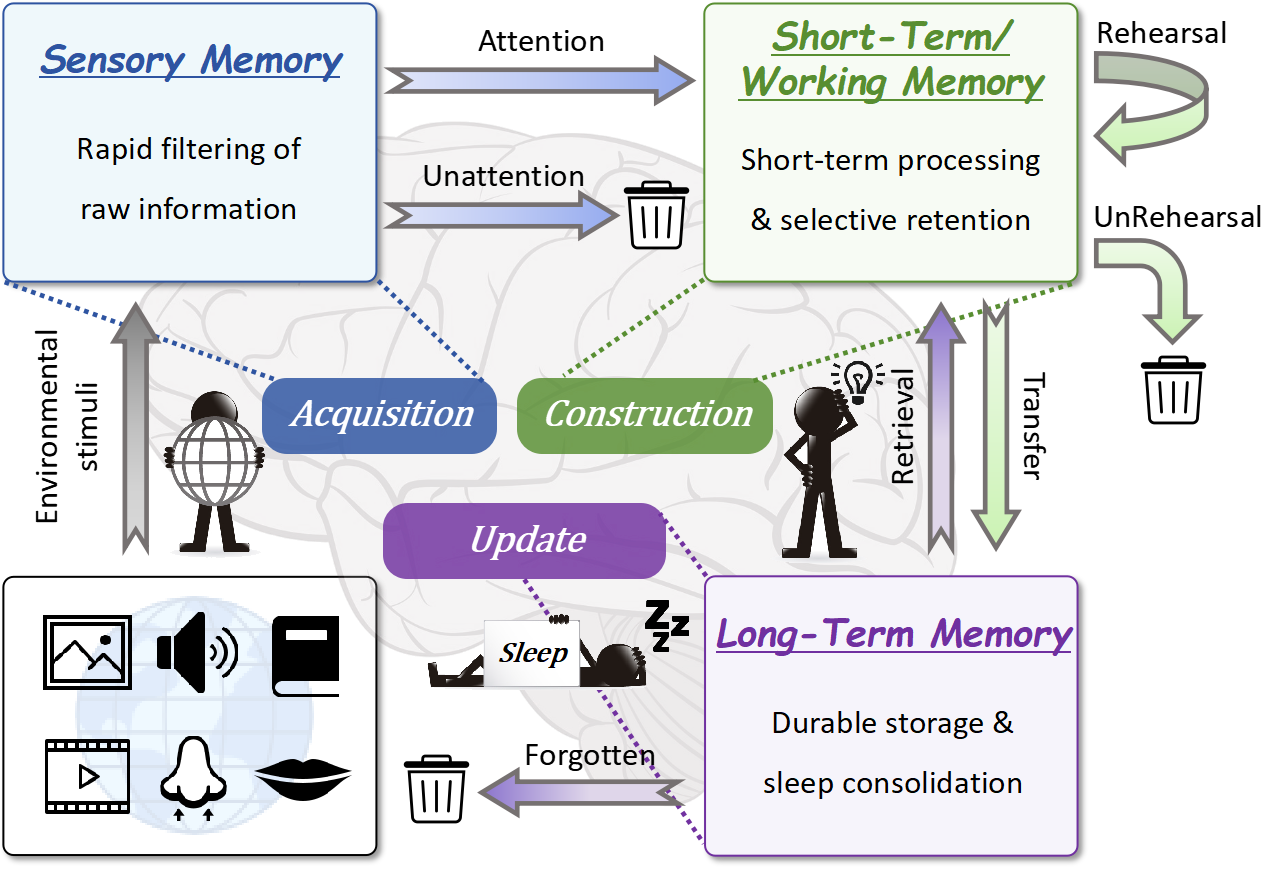
\includegraphics[width=0.94\linewidth]{figure/human.png}
%     \caption{Human memory system.}
%     \label{fig:human}
%     \vspace{-0.5cm}
% \end{wrapfigure}
% Following the Atkinson–Shiffrin human memory model~\citep{atkinson1968human}, raw environmental information in human brain is first briefly retained in \textit{sensory memory}, which enables rapid pre-attentive feature extraction and filtering, effectively serving as a form of pre-compression. 
% The processed input can then enter \textit{short-term memory} (STM), where information and interaction sequences are preserved for tens of seconds to minutes, supporting secondary filtering and more deliberate processing. 
% In contrast, \textit{long-term memory} (LTM) provides durable storage and undergoes continuous reorganization through updating, abstraction, and forgetting. 
% Importantly, \citet{rasch2013sleep} highlight that \textit{sleep plays a critical role in this reorganization}, as oscillatory activity during sleep facilitates the integration and consolidation of memory systems.

% Following the Atkinson–Shiffrin model~\citep{atkinson1968human}, raw information in humans is briefly stored in \textit{sensory memory} for rapid pre-attentive filtering.
% It then moves to \textit{short-term memory} (STM), retained for seconds to minutes for further filtering and processing.
% \textit{Long-term memory} (LTM) provides durable storage and is continuously reorganized through updating, abstraction, and forgetting.
% Besides, sleep also plays a critical role in this process, facilitating memory integration and consolidation~\citep{rasch2013sleep}.


\subsection{Limitations of Existing LLM Memory Systems}

Compared to human memory, current LLM memory systems are burdened by high maintenance costs, mainly due to three limitations:  
\textbf{1) Redundant Sensory Memory.} In current systems, $f_{\text{sum}}()$ and $f_{\text{gran}}(; g=\text{topic})$ are typically executed by calling stronger LLMs. 
Feeding raw data $D$ directly wastes resources and even weakens in-context learning due to redundancy. 
A key challenge is to design lightweight mechanisms that pre-compress inputs and apply pre-attention strategies to capture semantic units at different granularities efficiently.  
\textbf{2) Balancing Effectiveness and Efficiency in STM.} 
As shown in Figure~\ref{fig:motivation}, when input granularity is fixed, $D^{(g)}$ must pass through the entire pipeline. 
Excessively fine granularity increases latency and underutilizes STM capacity, whereas overly coarse granularity without semantic constraints or grouping may cause mixed or entangled semantics and topics, leading to inaccurate memory construction and loss of fine-grained details in subsequent processes. 
This calls for strategies that better balance effectiveness and efficiency in STM.  
\textbf{3) Inefficient LTM Updating.} 
Current $f_{\text{update}}()$ mechanisms face two main issues: (i) enforcing strict real-time updates at test time incurs significant latency, whereas STM can provide short-term context without immediate LTM updates; (ii) memory banks are updated sequentially due to ordering constraints (read-after-write/write-after-read), rather than being triggered dynamically. 
These limitations raise a research question: \emph{Can we design LLM memory that is both efficient and lightweight, inspired by human memory mechanisms?}



% This raises the question of whether LTM updates can be less tied to real-time triggers and sequential execution. 


% This process is analogous to how humans learn: when attending a lecture or reading, we selectively retain key points, jot down notes to extend our short-term retention, and even during sleep may vividly recall or reprocess what we studied earlier in the day as shown in Figure \ref{fig:human}.
% A research question arises: \emph{What insights can be drawn to align LLM memory with human memory in terms of efficiency and lightweight design?}
% In this work, we investigate three directions:  

% \noindent \textbf{Introduction of Sensory Memory.} 
% In current LLM memory, $f_{\text{sum}}()$ and $f_{\text{gran}}(; g=topic)$ are typically executed by invoking strengthen LLMs. 
% Directly feeding raw data $D$ from real-world scenarios into model wastes resources and even weakens its in-context ability due to redundant information. 
% Can we design a lightweight mechanism to first pre-compress raw information and employ a pre-attention strategy to efficiently capture semantic units at various granularities? 

% \begin{wrapfigure}{r}{0.5\columnwidth}
%     \vspace{-0.2cm}
%     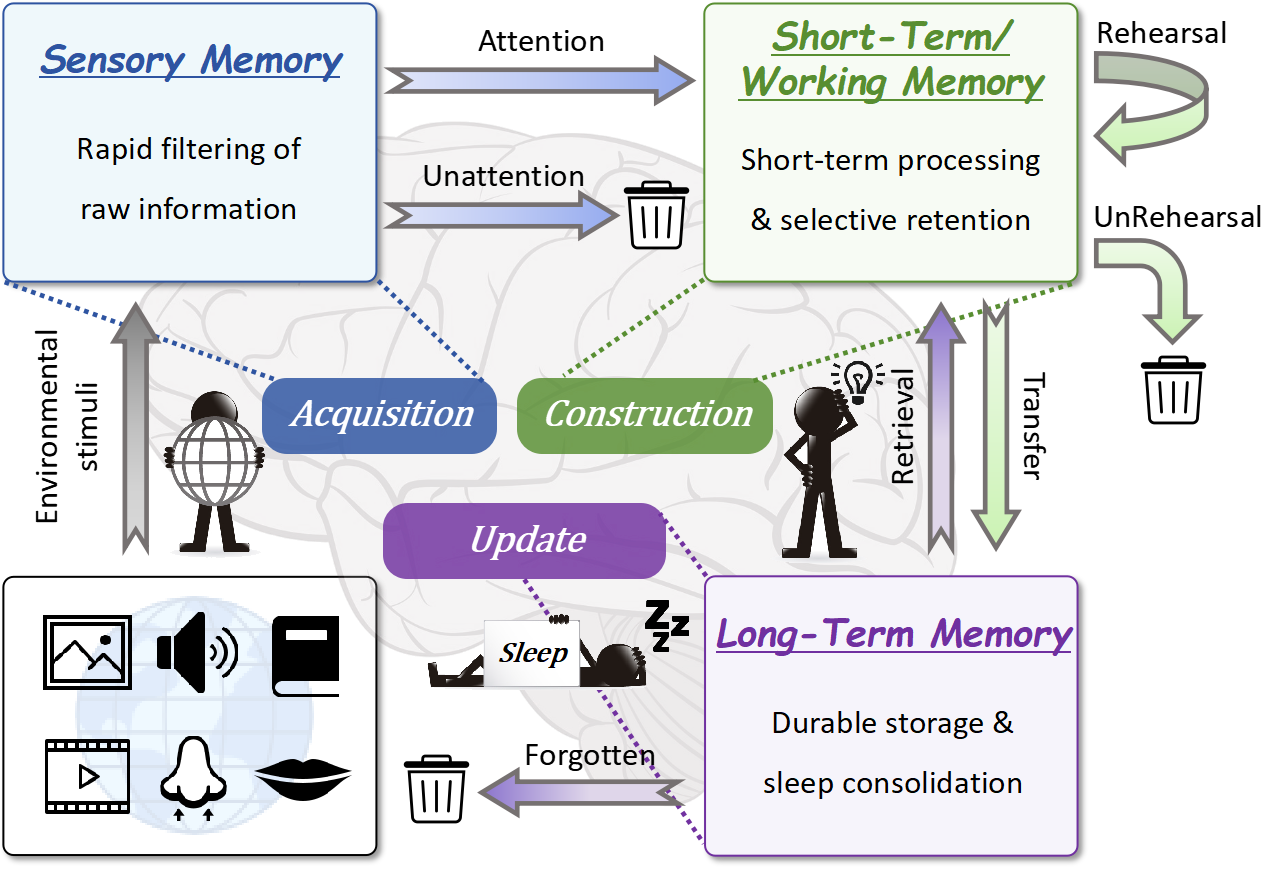
\includegraphics[width=0.94\linewidth]{figure/human.png}
%     \caption{Human memory system.}
%     \label{fig:human}
%     \vspace{-0.5cm}
% \end{wrapfigure}

% \noindent \textbf{Balancing Effectiveness and Efficiency in STM.} 
% In current memory frameworks, as shown in Figure~\ref{fig:motivation}, when the input granularity is fixed, $D(g)$ must sequentially pass through the entire pipeline. 
% If the granularity is too small, it results in significant latency across the data stream and underutilization of STM capacity. 
% If the granularity is too large, performance degrades due to an excessively long context.
% This calls for strategies to better balance performance and efficiency in STM design. 

% \noindent \textbf{Optimizing LTM Updating Mechanisms.}
% \label{LTM_motivation}
% The $f_{\text{update}}()$ of current LLM memory has two main limitations. 
% First, existing approaches enforce strict real-time LTM updates at test time, incurring substantial latency. 
% We argue that a practical LLM memory system should coordinate STM and LTM, where information in STM need not be immediately updated to LTM, as contextual information can be directly leveraged from STM.
% Second, memory bank updates are typically performed sequentially due to ordering constraints (read-after-write/write-after-read problem). 
% This raises the question of whether LTM updates can be less tied to real-time triggers and sequential execution. 